% !TEX encoding = UTF-8 Unicode
% !TEX spellcheck = en-US


% This is the root file of your thesis: thesis.tex
% A line starting with % is a comment. In some cases, I have included a command preceded by a %. You may activate the command by removing the %.

%%===================================
\documentclass[12pt]{report}
\usepackage{ramsstyle}
\usepackage{float}
\usepackage{graphicx}
\usepackage{wrapfig}
\usepackage{gensymb}
\usepackage{courier}
%%===================================
%Write the various parts of your thesis as separate files and include them into the main file by the command \include{name of included file}. When you compile the LaTeX file, you may choose which subfiles to include by the command

%\includeonly{chapter01,chapter02}

%%===================================
\begin{document}
% !TEX encoding = UTF-8 Unicode
%!TEX root = thesis.tex
% !TEX spellcheck = en-US

%This is the Titlepage
%%=========================================
\thispagestyle{empty}

\includegraphics[scale=1.1]{fig/NTNU}
\mbox{}\\[6pc]
\begin{center}
\Huge{Specification and First Prototype of Simulated Environment for Autonomous USV}\\[2pc]

\Large{Kjetil Save Børs-Lind}\\[1pc]
\large{August 2016}\\[2pc]

TTK4550 - Specialization Project\\
Department of Engineering Cybernetics\\
Norwegian University of Science and Technology
\end{center}
\vfill

\noindent Supervisor: Morten Breivik, ITK

\noindent Co-supervisor: Rein Anders Apeland, Kongsberg Maritime


 % This is the titlepage
\setcounter{page}{0}
\pagenumbering{roman}
% !TEX encoding = UTF-8 Unicode
%!TEX root = thesis.tex
% !TEX spellcheck = en-US
%%=========================================
\addcontentsline{toc}{section}{Preface}
\section*{Preface}
Some preface.\\[2cm]

\begin{center}
Trondheim, 2012-12-16\\[1pc]
(Your signature)\\[1pc]
Ola Nordmann
\end{center}
% !TEX encoding = UTF-8 Unicode
%!TEX root = thesis.tex
% !TEX spellcheck = en-US
%%=========================================
\addcontentsline{toc}{section}{Summary and Conclusions}
\section*{Summary and Conclusions}
Here you give a summary of your your work and your results. This is like a management summary and should be written in a clear and easy language, without many difficult terms and without abbreviations. Everything you present here must be treated in more detail in the main report. You should not give any references to the report in the summary -- just explain what you have done and what you have found out. The Summary and Conclusions should be no more than two pages.

You may assume that you have got three minutes to present to the Rector of NTNU  what you have done and what you have found out as part of your thesis. (He is an intelligent person, but does not know much about your field of expertise.)
\tableofcontents
\setcounter{page}{0}
\pagenumbering{arabic}

%Introduction
% !TEX encoding = UTF-8 Unicode
%!TEX root = thesis.tex
% !TEX spellcheck = en-US
%%=========================================
\chapter{Introduction}
The first chapter of a well-structured thesis is always an introduction, setting the scene with background, problem description, objectives, limitations, and then looking ahead to summarize what is in the rest of the report. This is the part that readers look at first---\emph{so make sure it hooks them!}

%%=========================================
\section{Background}
In this section, you should present the problem that you are going to investigate or analyze; why this problem is of interest; what has, so far, been done to solve the problem, and which parts of the problem that remain.

{\color{red}Below, I have set up some headings (subsection titles) without a number. These are included to help you remember to cover the related issues. The headings should be removed in your final print.}
%%=========================================
\subsection*{Problem Formulation}
You should define your problem in a clear an unambiguous way and explain why this is a problem, why it is of interest---and to whom. It is also important to delimit the problem area.
%%=========================================
\subsection*{Literature Survey}
You should here present the main books and articles that treat problems that are similar to what  you are studying. If you,  later in your thesis, describe the ``state of the art'' -- with a detailed literature survey, you may just give a very brief survey here (approx. a quarter of a page). If this is the only literature survey, you need to go into more details. An objective of the literature survey is to show the reader that you are familiar with the main literature within your field of research -- so that you do not ``reinvent the wheel.''


References to literature can be given in two different ways:
\begin{itemize}
\item As an \emph{explicit} reference: It is shown by \citet{lundteigen08} and partly also by \citet{rausand14}  that \ldots.
\item As an \emph{implicit} reference: It is shown \citep[e.g., see][Chap. 4]{rausand04} that \ldots.
\end{itemize}
In the example above, we have used ``author-year'' references, which is the preferred format. 
\begin{remark}
Following agreement with your supervisor, you may also refer by numbers, for example,  [1]. To do this, open the file \texttt{ramsstyle.sty} and  comment out (by \%) the command \texttt{$\backslash$usepackage\{natbib\}} and un-comment the corresponding command \texttt{$\backslash$usepackage[numbers]\{natbib\}}.\footnote{Notice the strange way we have to write the ``backslash'' in the text. This is because the ``backslash'' is a command in \LaTeX.}
\end{remark}
 You may include a link to the Internet in the text or in a footnote by using a command like: \url{http://www.ntnu.edu/ross}. 

When you refer to the scientific literature, you should always write in \emph{present} tense. Example: \citet{rausand04} show that \ldots.

\begin{remark}
Hyperlinks are included by the command \texttt{$\backslash$usepackage\{hyperref}\} in \texttt{ramsstyle.sty}. If you feel that the hyperlinks are disturbing when you enter the text, or want to avoid the hyperlinks in printed text, you may either comment out or edit this command in \texttt{ramsstyle.sty}.
\end{remark}
%%=========================================
\subsection*{What Remains to be Done?}
After you have defined and delimited your problem -- and presented the relevant results found in the literature within this field, you should sum up which parts of the problem that remain to be solved.
%%=========================================
\section{Objectives}
The main objectives of this Master's project are
\begin{enumerate}
\item This is the first objective
\item This is the second objective
\item This is the third objective
\item More objectives
\end{enumerate}

The objectives shall be written as \emph{fundamental objectives} telling what to do and not \emph{means objectives} telling how to do it.

All objectives shall be stated such that we, after having read the thesis, can see whether or not you have met the objective. ``To become familiar with \ldots'' is therefore not a suitable objective.

%%=========================================
\section{Limitations}
In this section you describe the limitations of your study. These may be related to the study object (physical limitations, operational limitations), to the environmental and operational conditions, to the thoroughness of the analysis, and so on.
%%=========================================
\section{Approach}
Here you should describe the (scientific) approach that you will use to solve the problem and meet your objectives. You should specify the approach for each objective.

If there are any ethical problems related to your approach, these should be highlighted and discussed.
%%=========================================
\section{Structure of the Report}
The rest of the report is organized as follows. Chapter 2 gives an introduction to \ldots

\begin{remark}
Notice that chapter and section headings shall be written in lowercase, but that all main words should start with a capital letter.
\end{remark}


The report should be no longer than \underline{60 pages} in this format (+ the CV).

%Existing solutions
% !TEX encoding = UTF-8 Unicode
%!TEX root = thesis.tex
% !TEX spellcheck = en-US
%%=========================================
\chapter{Existing Solutions}


\section{CyberSea Simulator}
The CyberSea Simulator developed by Marine Cybernetics is a simulator for HIL testing of Dynamic Positioning (DP) systems.

Key points from [\cite{HILtestingDP}]:
\begin{itemize}
\item Capabilities for data logging and real-time presentation of results
\item Emphasis on vessel dynamics and accurate simulation of vessel motion at low speed ( < 3kts, wave, wind and current loads (of course, because of DP) in six degrees of freedom "using a nonlinear rigid-body model of the vessel".
\item Several options for interface between HIL Simulator and Computer Control System ("Analog, digital, serial/NMEA protocol", normal network protocol or "dedicated test I/O built into the DP computer system").
\item Generation of realistic signals from all the common sensors and position reference systems (such as "Gyro-compasses, VRUs, wind sensors, thruster feedback [...], power feedback from thrusters, switchboard and generator sets") used in modern DP technology "contaminated with typical noise levels".
\item Advanced generation of GNSS signals with possibility of simulating a broad specter of common failure modes.
\end{itemize}


\section{MSS (Fossen)}

\section{MCSim (Marine Cybernetics)}

\section{Gazebo (ROS)}

%Sensors
% !TEX encoding = UTF-8 Unicode
%!TEX root = thesis.tex
% !TEX spellcheck = en-US
%%=========================================
\chapter{Implementation and Simulation of Sensors}
Using electronic nautical charts (ENC), information about other simulated agents and 3D models of installations in sea it is possible to generate realistic sensor data for HIL simulations. This section contains an overview of the implementation of important sensors used on Odin and a brief discussion about how sensor data can be simulated. The Inertial Measurement Unit (IMU) is documented in (\textbf{Evens rapport, trenger referanse?}).

\section{Sensors for Environmental Analysis Implemented on Odin}
\label{SensorOverview}
In section \ref{SensorOverview} a brief overview of the sensors on Odin used for situational awareness above the surface are presented. The overall layout of sensors and system architecture are visualized in Figure \ref{fig:systemArchitecture}.

\begin{figure}[H]
	\begin{center}
		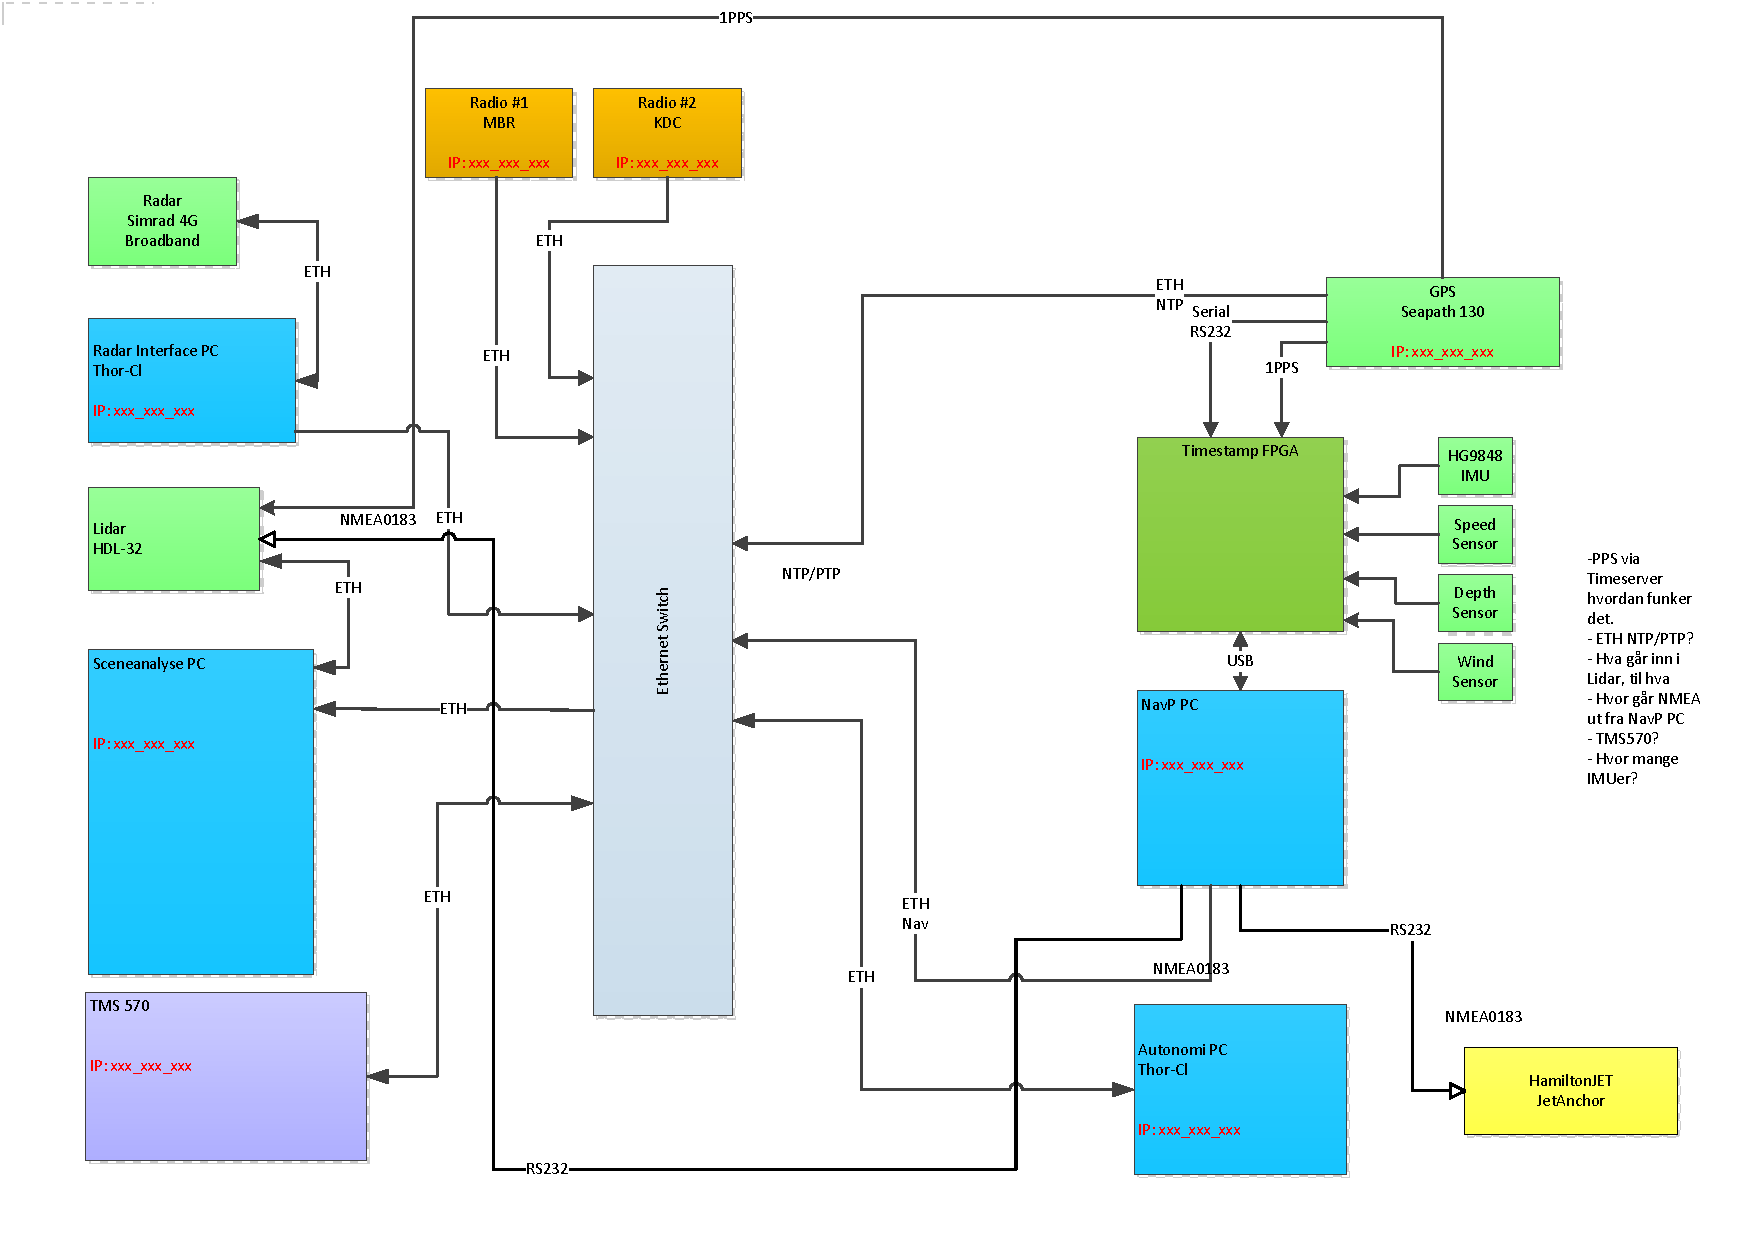
\includegraphics[width = 1\linewidth]{fig/SystemarkitekturOdin.pdf}
		\caption{\textit{Visualization of system architecture and network layout on Odin, including sensors and processing units.} \textbf{A better figure should be made when the final layout is determined!}}
		\label{fig:systemArchitecture}
	\end{center}
\end{figure}

\subsection{Seapath 134 GPS}
The GPS used on Odin is the Seapath 134 developed by Kongsberg Seatex. Combining GNSS signals and IMU data the Seapath 134 gives highly accurate heading, position, heave, roll and pitch measurements (\cite{SeapathManual}). Data is transmitted via standard NMEA 0183 protocol (\cite{NMEAmanual}) over a serial RS232 cable for interpretation by the control system. \textbf{Short introduction and small example of NMEA protocol should come here.}

\begin{figure}[H]
	\begin{center}
		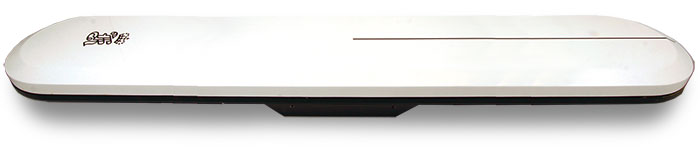
\includegraphics[width = 0.7\linewidth]{fig/Seapath130.jpg}
		\caption{\textit{The Seapath 134 developed by Kongsberg Seatex is used on Odin for position, heading and attitude measurements.}}
		\label{fig:seapath130}
	\end{center}
\end{figure}

\subsection{Radar}
\begin{wrapfigure}[7]{r}{0.3\textwidth}
	\vspace{-30pt}
	\begin{center}
		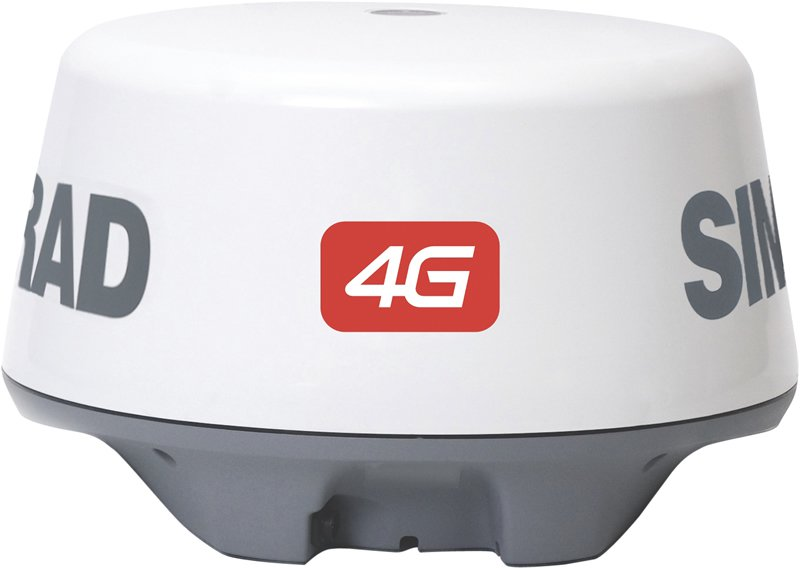
\includegraphics[width= 0.9\linewidth]{fig/navico4G}
		\vspace{-10pt}
		\caption{\it{Simrad Broadband 4G radar used on Odin.}}
		\label{fig:navico4G}
	\end{center}	
\end{wrapfigure}
The radar used on Odin is a Simrad Broadband 4G with range from 200 feet to 32 nautical miles and 48 RPM sweep  rate (\cite{simradBrochure}). The radar communicates directly with the \textit{Radar Interface PC} as seen in Figure \ref{fig:systemArchitecture}. Automatic Radar Plotting Aid (ARPA) (\cite{ARPAmanual}) is used for target tracking and analysis in the radar interface. It is assumed that the radar interface including the ARPA functionality is well tested and that the output from \textit{Radar Interface PC} is predictable and well documented, possibly following some NMEA like protocol. At the current time the details of the transaction of this information is not yet decided. Processed target and surroundings data is transmitted via Ethernet and is assumed to at least include information about target position, heading and speed. Other possibly available data might be time and point of collision, radar cross section (or other target size information) and current noise conditions.\\


\newpage
\subsection{Velodyne LiDAR HDL-32E}
\begin{wrapfigure}[14]{l}{0.3\textwidth}
	\vspace{-30pt}
	\begin{center}
		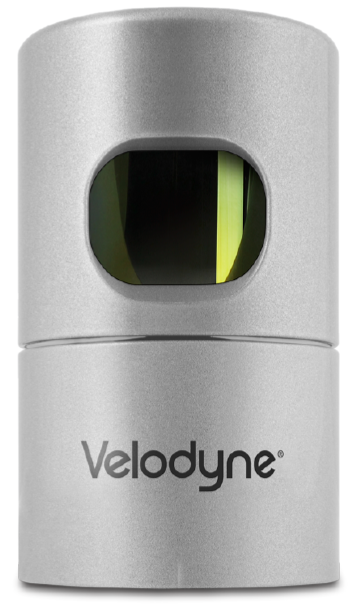
\includegraphics[width= 0.9\linewidth]{fig/VelodyneHDL32Ecase}
		\vspace{-20pt}
		\caption{\it{Velodyne LiDAR HDL-32E used on Odin for above-the-surface 3D analysis.}}
		\label{fig:velodyneCasing}
	\end{center}
	
\end{wrapfigure}
For analysis of the nearby environment above the surface a LiDAR is used to create a 3D point cloud. The model used on Odin is a Velodyne HDL-32E as seen in Figure \ref{fig:velodyneCasing}. A LiDAR can measure the distance to points around the sensor by firing a laser and measure the time it takes for the light to return. The distance is then saved along with the horizontal and vertical angle of the laser, so that the positions of the measured points can be used to generate a 3D model of the nearby environment. Velodyne HDL-32E generates 700,000 points per second with $\pm2$cm accuracy at 80m-100m range. The LiDAR spins around the vertical axis to achieve a $360\degree$ horizontal field of view (FOV), and a combination of 32 lasers stacked vertically yields a $40\degree$ vertical FOV ($+10\degree$ to $-30\degree$). An external GPS should be connected to the LiDAR for time pulse synchronization.

Uncalibrated point cloud data packets are transmitted from the LiDAR over a standard Ethernet cable using UDP. The packet format is well documented in the user manual so that they should be easy to decompose by a custom made point cloud processing unit. A calibration table must be used for vertical correction for each laser. This table is included on a CD delivered with the HDL-32E.

The LiDAR sweeps are processed by \textit{Sceneanalys PC} as seen in Figure \ref{fig:systemArchitecture}. The data is stored in a ROS structure called \texttt{grid\_map} and sent to the motion planning module in \textit{Autonomi PC} (Figure \ref{fig:systemArchitecture}). Detected objects are planned to be put in ROS messages containing information about relative position, speed, heading, latitude/longitide and detection probability.


\section{Simulation of Sensor Data from Virtual Environment}
The feasibility of simulating realistic sensor data from a virtual environment will be discussed in this section, as well as complexity and benefits regarding simulation of raw versus preprocessed sensor data. Information, hardware and software needed to generate data from each sensor will also be discussed.

\subsection{Simulating Data from GPS}
As the data output of the Seapath 134 follows the well documented NMEA0183 protocol it should be feasible to generate these data based on knowledge of position, speed, heading and attitude. This information should be a result of simulating the boats motion in the virtual environment and is thereby easily accessible.
\remark{ In the system architecture (Figure \ref{fig:systemArchitecture}) of Odin the GPS is used for time synchronization of the entire system. It is assumed that the HIL setup is synchronized in time using either NTP or PTP network timing. A real or simulated GPS time synchronization signal is therefore not considered necessary in the scope of this project. 

\subsection{Simulating Data from Radar}
Assuming predictable and well documented data output from \textit{Radar Interface PC} (Figure \ref{fig:systemArchitecture}) it should be feasible to simulate output from this subsystem given information about simulated targets around Odin. Simulating raw data from the radar, i.e simulating the exact radio signal reflected from the target, is considered too complex to stay within the scope of this project. This is because it requires too detailed information about everything from the target shape, weather conditions and the specific radar in use as well as a deep understanding of radar technology. It is thereby determined that only preprocessed data from the \textit{Radar Interface PC} will be simulated. To simulate realistic output the following points should be considered:

\begin{itemize}
	\item Radar blind zones minimum detection range.
	\item Radar range being dependent on weather conditions. 
	\item Target detection dependent on the shape and orientation of target.
	\item During precipitation clutter a target may or may not be detected. A solution could be to use a randomize function to determine if a target should be detected or not. In that case, reproducibility of simulation might be more difficult.
	\item Accuracy of the implemented radar and how to model errors resulting from inaccuracy. \cite{ARPAmanual} gives great details about possible errors.
\end{itemize}

\subsection{Simulating Data from LiDAR}
The protocol of the data transfer from Velodyne HDL-32E is well documented. Given a 3D model of the surrounding environment with easy access to angle and distance calculations it should be feasible to generate a realistic point cloud. The point cloud can be represented as data packets using the HDL-32E protocol and sent over Ethernet to the interface between HIL simulator and the control system. This way it would be possible to simulate raw sensor readings from the HDL-32E. This is assumed to be beneficial to the developers of the simulated vehicle as a larger chain of HW/SW can be tested in the simulated environment. A challenge with this approach is to simulate realistic sensor readings during rainy conditions and other environmental disturbances. A solution could be to use randomized noise added to the simulated measurements. A deterministic randomize function should be used to ensure reproducibility of the simulations. 3D modeling of the surrounding environment might also be computationally challenging. More research should be done to investigate the feasibility of this.\\ 
\\
As shown in Figure \ref{fig:systemArchitecture}, the data from the LiDAR is processed by the \textit{Sceneanalyse PC}. If this module is well tested, or the 3D processing of the surrounding environment is too computationally heavy, it might be more convenient to simulate the output from this PC directly without going through the steps of generating a point cloud. \textbf{The output from \textit{Sceneanalyse PC} is what? Possibly strings with information about nearby targets? Would be easy to generate.}









%Simulator interface
% !TEX encoding = UTF-8 Unicode
%!TEX root = thesis.tex
% !TEX spellcheck = en-US
%%=========================================
\chapter{Interface between Simulator and Control System}
This chapter will aim to decide an overall layout of the interface between the HIL Simulator and the USV control system to be tested. It will also be suggested an overview of the information flow between important modules of the simulator. Only a general layout will be suggested as the primary simulation target (Odin) is still under development and many details about the HW and SW solutions on board the USV are yet to be decided.

\newpage
\section{Overview of the Simulation Setup}
\begin{wrapfigure}[21]{r}{0.6\textwidth}
	\vspace{-40pt}
	\begin{center}
		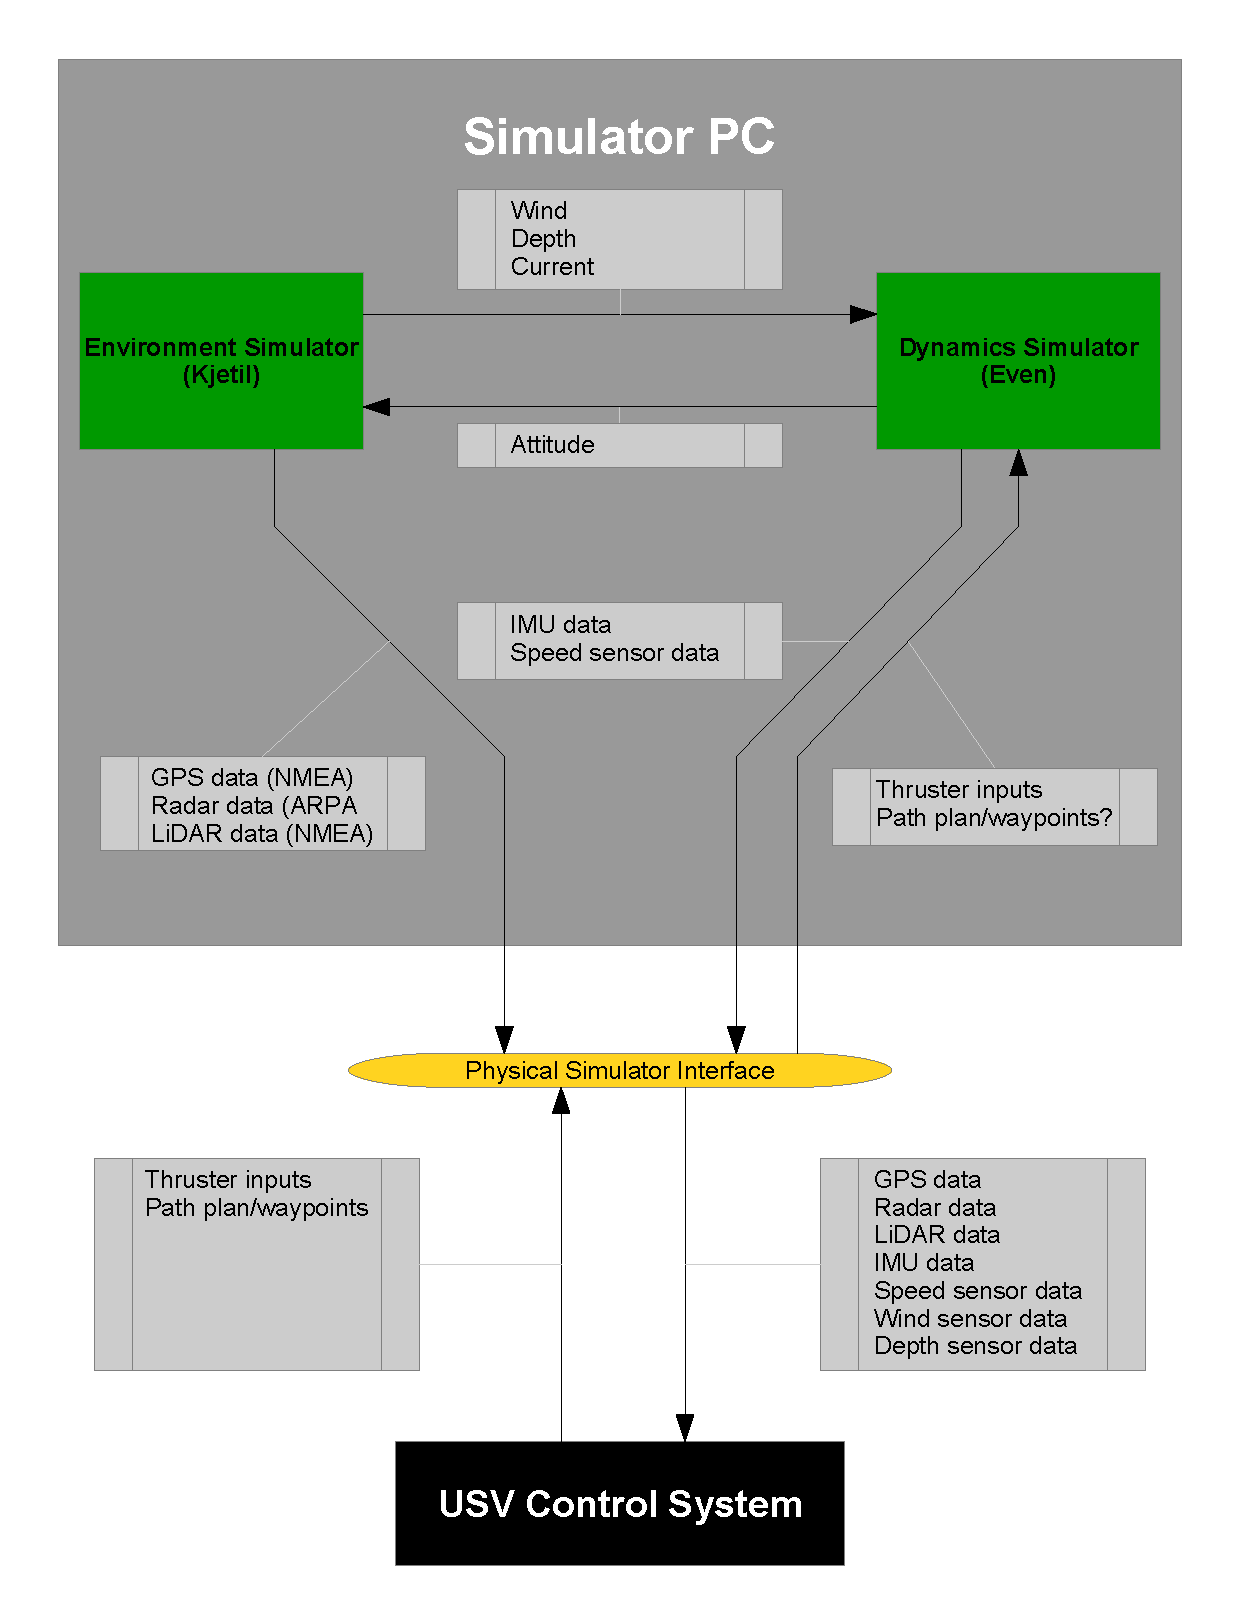
\includegraphics[width= \linewidth]{fig/Interface.pdf}
		\vspace{-40pt}
		\caption{\it{General overview of the planned design of the HIL Simulation setup. The overview includes general information flow between the USV control system, simulator and main software modules.}}
		\label{fig:simLayout}
	\end{center}	
\end{wrapfigure}

The HIL Simulator should be run on a single laptop. The operating system (OS) should be Ubuntu to be able to utilize ROS functionality during simulation. The task of developing the simulator is divided in two projects- and master thesis's: one for the simulation of the surrounding environment around the USV (this project) and one for the simulation of the USV dynamics (\cite{even}). The dividing in two tasks makes it natural to split the simulation software in two main modules: Dynamics and Environment as seen in Figure \ref{fig:simLayout}. The boats attitude and movement at any time are calculated in the Dynamics module. This information should be sent to the Environment module which decides the USV's global position in the simulation environment. Weather conditions such as wind and current are decided in the Environment module and sent to the Dynamics module which calculates how these factors influences the motion of the USV. The two modules, knowing everything about the surroundings and attitude of the USV, generates appropriate sensor data and sends this to the physical interface connecting the HIL Simulator to the USV control system. 

\subsection{Information Flow Between Software Modules}


\section{Physical Interface}
Too early to decide the details of this.



%Logging and visualization of simulation (possibly implementation in C++)
% !TEX encoding = UTF-8 Unicode
%!TEX root = thesis.tex
% !TEX spellcheck = en-US
%%=========================================
\chapter{Logging and Visualization of Simulation}

\section{Logging}

\section{Visualization}

\section{C++ example?}





%Use of model in automatic testing invironment (ROS)
% !TEX encoding = UTF-8 Unicode
%!TEX root = thesis.tex
% !TEX spellcheck = en-US
%%=========================================
\chapter{Use of Model in Autonomous Testing Environment (ROS)}





%Other agents
% !TEX encoding = UTF-8 Unicode
%!TEX root = thesis.tex
% !TEX spellcheck = en-US
%%=========================================
\chapter{Other Agents and their Behavior as Part of Simulated Environment}

\section{Possible Agents}
\subsection{Ships}
\subsection{Small Boats}

\section{Pros and Cons of Agents Behavior}
\subsection{Reactivity?}
\subsection{Predictability}
\subsection{Possibility of Repeating Scenario}


%Conclusion and further work
% !TEX encoding = UTF-8 Unicode
%!TEX root = thesis.tex
% !TEX spellcheck = en-US
%%=========================================
\chapter[Summary]{Summary and Recommendations for Further Work}

%%=========================================
\section{Summary and Conclusions}

%%=========================================
\section{Discussion}
%%=========================================
\section{Recommendations for Further Work}

% Include more chapters as required.
%%=========================================
\appendix
% !TEX encoding = UTF-8 Unicode
%!TEX root = thesis.tex
% !TEX spellcheck = en-US
%%=========================================

\chapter{Acronyms}
\begin{description}
\item[FTA] Fault tree analysis
\item[MTTF] Mean time to failure
\item[RAMS] Reliability, availability, maintainability, and safety
\end{description}
% !TEX encoding = UTF-8 Unicode
%!TEX root = thesis.tex
% !TEX spellcheck = en-US
%%=========================================

\chapter{Additional Information}
This is an example of an Appendix. You can write an Appendix in the same way as a chapter, with sections, subsections, and so on.

%%=========================================
\section{Introduction}

%%=========================================
\subsection{More Details}
% Include more appendices as required.
%%=========================================
\bibliographystyle{apa}
\addcontentsline{toc}{chapter}{\bibname}
\bibliography{refs}  

\end{document}
